\chapter{Le šī`isme ou l'islam sous un autre visage}

Avant d'exposer les doctrines et pratiques propres au šī`isme, je vous
propose de regarder cette petite vidéo d'un peu moins de 10 minutes.
Elle sera une bonne introduction de ce qui est dit du šī`isme. Vous
devrez pouvoir répondre aux questions de l'encadré ci-dessous. Pour
autant si ce cours va permettre de préciser les informations
mentionnées, il en révélera aussi quelques dimensions que ne signerait
pas un šī`ite. C'est tout le problème de l'imbrication entre la
théologie et l'histoire.

\paragraph{Questions}

\begin{enumerate}
\def\labelenumi{\arabic{enumi}.}
\item
  D'où vient le mot šī`ite~?
\item
  Quel est l'évènement fondateur du šī`isme~?
\item
  Quelles sont les principales villes saintes du šī`isme~?
\item
  Le šī`isme est-il un phénomène spécifiquement persan~?
\end{enumerate}


En raison de la révolution iranienne en Iran en 1979, l'image du šī`isme
véhiculée en Occident a été bien souvent celle de croyances
obscurantistes, d'intolérance, de régression, de violence politique. En
2004, Mohammad Amir-Moezzi et Christian Jambet pouvaient écrire~dans un
ouvrage de grande qualité pédagogique, \emph{Qu'est-ce que le
shî'ism~?}~: «~le shî'isme est une figure de style pour `islam radical',
voire pour `islam terroriste'~»\sn{Mohammad-Ali
  \textsc{Amir-Moezzi}, Christian Jambet, \emph{Qu'est-ce que le
  shî'isme~?,} Paris, Fayard, 2004.} (p. 12).

Cette image est en train de disparaître. Le départ de la scène politique
du président Mahmoud Ahmadinejad après deux mandats (2005-2013) et le
climat de détente avec les États-Unis y est sans doute pour beaucoup.
Sans compter, bien sûr, Al-Qaida, Daesh, autant d'émanations d'un islam
politique extrémiste instrumentalisant le meurtre et la terreur, qui ne
sont pas šī`ites mais sunnites. J'ajouterai que le travail de
vulgarisation des islamologues sur le šī`isme, d'historicisation, de
contextualisation de la République islamique d'Iran et de l'idéologie de
l'ayatollah Khomeiny par rapport à ce courant musulman qui prend son
origine au premier siècle de l'islam y a aussi sa part. Le cinéma
contribue aussi à donner une autre image de la société iranienne.

Mais fondamentalement, qu'est-ce que le \emph{šī`isme}~? S'agit-il d'un
autre islam que le sunnisme ou du même islam mais avec un visage
différent~? Les oppositions politiques au cours de l'histoire, les
polémiques virulentes notamment durant la période des empires ottomans
et safavides, donnent l'image de deux irréductibles, de deux
irréconciliables, de deux frères ennemis. Avoir conscience et
connaissance de la singularité du \emph{šī`isme} ne doit pas faire pour
autant oublier que les šī`ites se disent musulmans et qu'il existe des
penseurs travaillant pour un «~œcuménisme~» entre sunnisme et šī`isme.
Telle est l'approche par exemple de Seyyed Hossein Nasr qui présente le
šī`isme comme «~une affirmation d'une dimension particulière de l'islam
qui est centrale et qui est considérée par les \emph{šī`ites} comme
faisant partie de l'islam en tant que tel. Il n'a pas été un mouvement
qui a d'une certaine manière détruit l'unité de l'islam, mais un de ceux
qui a ajouté à la richesse du déploiement historique et de la diffusion
du message coranique~»\sn{Seyyed Hossein Nasr dans Sayyid Muḥammad
  Husayn Ṭabāṭabā'ī, \emph{Shi‛ite Islam} , translated and edited by
  Seyyed Hossein Nasr , Albany, State University of New York Press,
  1975, p.7.}.

Certes, il existe des aspects historiques et religieux du šī`isme qui
contredisent le sunnisme, mais ce professeur iranien de philosophie
appelle à y voir le signe d'une pluralité d'interprétations possibles.
Il ne s'agit pas d'élaborer un dénominateur commun mais de voir que
l'unité embrasse les différentes «~facettes de l'islam~». Pour lui,
c'est dans la mystique, la spiritualité, l'ésotérisme qu'il est possible
de transcender, de dépasser les différences et de trouver l'unité. 


Mais avant de voir comment sunnisme et šī`isme relèvent tous deux de la
même unité qu'est l'umma, la communauté musulmane, quels sont les
éléments fondamentaux d'histoire, de doctrines et de pratique du
šī`isme~?


\vide{i.-les-fondations-du-ux161ux12bisme-histoire}{%
\section{Les fondations du šī`isme~: histoire
}\label{i.-les-fondations-du-ux161ux12bisme-histoire}}

\vide{origine-du-ux161ux12bisme-la-question-de-la-succession}{%
\subsection{Origine du šī`isme~: la
question de la
succession}\label{origine-du-ux161ux12bisme-la-question-de-la-succession}}

\vide{le-siisme-une-prophuxe9tologie.-il-y-a-une-sur-lincarnation.-facile-le-dialogue.}{%
\mn{Le si'isme, une prophétologie. Il y a une sur
l'incarnation. Facile le
dialogue.}\label{le-siisme-une-prophuxe9tologie.-il-y-a-une-sur-lincarnation.-facile-le-dialogue.}}

\mn{
Kerbala~: c'est la ville qui n'a pas défendu les enfants du prophète.
Rédemption par le sang.}
Comme mentionné dans la vidéo, le terme arabe \emph{šī`a} signifie
parti, adhérent, fidèle. S'il y est mentionné que l'acte de naissance du
šī`isme est la bataille de Kerbala, pour les šī`ites, le šī`isme
existait du vivant de Muḥammad.

`Alī en effet est le fils d'Abū Ṭālib, l'oncle paternel de Muḥammad. Il
est un des premiers convertis à l'islam. La tradition sunnite mentionne
que le Prophète lui avait confié (amāna) les biens des personnes dont il
était le représentant commercial et financier peu avant l'Hégire, que le
soir de l'Hégire, lorsqu'il quitta La Mecque, `Alī dormit dans son lit,
qu'il épousa Fāṭima, l'une des filles du Prophète.

Fāṭima joue un rôle très important dans l'histoire du šī`isme. Elle
décède à l'âge de 28 ans et `Alī n'épousera aucune autre femme. Il
semble, d'après les traditions šī`ites que Muḥammad avait imposé à son
gendre la monogamie pour sa fille Fāṭima. Elle aurait aussi obtenu de
son père l'autorisation d'aller prier sur les tombes de ceux qui avaient
été tués au cours des batailles.

À la mort du Prophète s'est posée la question de savoir qui allait
succéder à Muḥammad. Pour `Alī et ses partisans, Muḥammad a désigné son
successeur de son vivant. En effet, peu de temps avant sa mort, en 632,
Muḥammad se rendit à Ġadir Ḫumm~: c'est le pèlerinage d'adieu (Ḥaǧǧa
al-widā'). Il y reçut le verset suivant~: \emph{«~O Messager, transmets
ce qui t'a été descendu de la part de ton Seigneur. Si tu ne le faisais
pas, alors tu n'aurais pas communiqué Son message. Et Dieu te protégera
des gens. Certes, Dieu ne guide pas les gens mécréants.~» (Coran,
5:67).}

Par la suite, selon les šī`ites, Muḥammad déclara~: «~Man kuntu Mawlāhu,
fahaza `Alī mawlāhu~» c'est-à-dire~: «~Qui me reconnaît comme son Mawlā
(maître, guide), doit reconnaître `Ali comme son Mawlā ~».

\vide{section-44}{%
{{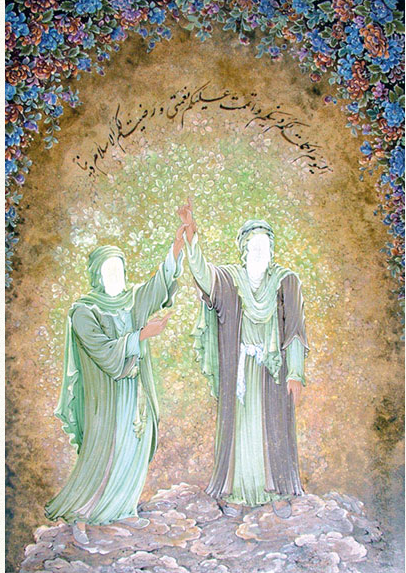
\includegraphics[width=1.35188in,height=1.90972in]{Images/image078.png}}{}}\label{section-44}}


\mn{{{Ġadir-e Khumm et la
désignation de l'Imâm `Alī}}
}


\mn{œuvre de Rezâ
Badr-os-Samâ'}

Mais pour certains des compagnons du Prophète, cette désignation n'a
jamais été officialisée et selon les mœurs tribales, il convient donc de
procéder à son élection.

Mais `Alī est écarté du collège électoral.

La tribu des Qurayš élit Abū Bakr, vieux compagnon et un des beaux-pères
de Muhammad~: il devint le 1\textsuperscript{er} calife (khalîfa).

`Alī fera acte d'allégeance, il se soumet à ce choix signifiant son
désir de maintenir l'unité de l'\emph{umma}.

À la mort d'Abū Bakr, `Umar devient le 2\textsuperscript{ème} calife
puisqu'il avait été désigné de manière explicite (\emph{naṣṣ}). `Alī
accepte.

`Umar annonce qu'à sa mort, son successeur devra être choisi parmi les
membres d'un collège électoral qu'il a lui-même nommés. `Alī en fait
partie. À la mort de `Umar, c'est `Uṯmān qui est choisi. Accusé de
népotisme, il est assassiné.

`Alī devient alors le 4\textsuperscript{ème} calife (656-661) attestant
ainsi de ses qualités vertueuses et de la suprématie de l'imamat sur les
manigances politiques mondaines.

Pour autant, deux anciens compagnons du Prophète n'ayant pas vu leur
appétit politique satisfait -- ils souhaitaient être gouverneurs de Kūfa
et Baṣra -- s'associèrent à `Ā'iša, fille d'Abū Bakr et veuve du
Prophète, pour lever une armée contre `Alī. C'est la bataille du chameau
de 657. On l'appelle ainsi parce que `Ā'iša qui était présente, était
montée sur un chameau\ldots{} Son armée fut mise en défaite.





\mn{On voit ici `Ā'iša sur son chameau et dans son baldaquin}



Mais en Syrie, Mu`āwiya, parent de `Uṯmān, mena aussi une guerre. C'est
la bataille de Ṣiffīn. Alors qu'elle tournait à l'avantage de `Alī,
Mu`āwiya proposa un arbitrage sur le livre sacré. `Alī accepte. Nombre
de ses soldats se soulèvent considérant qu'il n'avait pas à accepter
l'arbitrage et que Dieu avait déjà rendu son jugement par la victoire
qui se manifestait. `Alī doit mener combat contre ces rebelles (ce sont
les ḫariǧites), alors que Mu`āwiya se fait proclamer calife à Jérusalem
en 660~!

`Alī est assassiné par un ḫarigite à Kūfa en 661.

Pour les sunnites, il n'avait pas de successeur tandis que les šī`ites
affirment qu'il avait nommé son fils aîné, al-Ḥasān.

\vide{la-guxe9nuxe9alogie-du-ux161ux12bisme}{%
\subsection{La généalogie du
šī`isme}\label{la-guxe9nuxe9alogie-du-ux161ux12bisme}}

La généalogie est sujet à controverses et divergences ce qui explique la
multiplication des šī`ismes\textbf{.} On dénombre une centaine de
lignées à la fin du premier siècle de l'Hégire.

Les jours de naissances des membres de la famille de `Alī sont des fêtes
religieuses. Les jours anniversaires de leur mort, des journées de
deuil. Leurs tombes sont des lieux de pèlerinage~: les cités où elles se
trouvent sont des villes saintes.

Elle est un peu subtile, chaque imām mériterait un chapitre\ldots{}
entre son enseignement, les histoires, les légendes, leur assassinat --
souvent empoisonné -- sans compter qu'au sein même du šī`isme, les
généalogies, les filiations ne sont pas les mêmes, que certains ne
reconnaissent que quatre imāms, d'autres sept, d'autres douze, que ce ne
sont pas toujours les mêmes\ldots{} qu'il y a donc une multitude de
branches šī`ites\ldots{} Bref, je retiens surtout le šī`isme majoritaire
dit duodécimain, car il reconnaît 12 imāms. Vous en trouverez en annexe
la liste avec leurs noms et quelques caractéristiques. Si vous avez la
curiosité de regarder le douzième, vous voyez que n'est pas indiquée la
date de sa mort. D'après vous, est-ce parce que l'on ne la connaît pas,
ou est-ce pour une autre raison~? La réponse dans la suite du cours. Bon
travail.

\vide{alux12b-et-fux101tima}{%
\subsubsection{`Alī et Fātima}\label{alux12b-et-fux101tima}}

`Alī joue donc dans le šī`isme un rôle important. Il est à la tête de
presque toutes les chaînes de transmission, il est considéré ~comme un
maître spirituel. On lui attribue deux livres~: \emph{Nahj al-balâgha}
(La Voie de la maturité)~et \emph{Dîwân}, un recueil de poèmes.

Quant à Fātima, elle est la sainte la plus vénérée du šī`isme\textbf{.}
Sa tombe est à Médine (il y en a trois\ldots{} dans le doute, on les
garde toutes les trois).

Fātima est la mère de toute la lignée des imāms. Elle représente ce qui
relie Muhammad à `Ali, la lettre et l'esprit. Elle est dite \emph{maǧma`
al-nūrayn} (le Confluent des Deux Lumières), celle de la prophétie et de
l'imamat. Elle a une mission d'intercession et de protection jusqu'à la
fin des temps. Immaculée, Vierge malgré son mariage, elle est aussi
reine du ciel. Un parallèle avec Mariam (Marie), la mère de Jésus est
établi par la tradition šī`ite elle-même \sn{Tahani Sabri,
  «~L'hagiographie de Fāṭima d'après le \emph{biḥār al-anwār}~», École
  des Hautes Études en Sciences Sociales, thèse de doctorat sous la
  direction de Henry Corbin, 1969.}.

\vide{al-hasan-fils-de-aluxee}{%
\subsubsection{Al-Hasan, fils de
`Alî}\label{al-hasan-fils-de-aluxee}}

C'est un petit-fils du Prophète. Il y a des récits touchant d'affection
tendre.

Al-Ḥasan abdiqua le califat devant l'hostilité de Mu`āwiya. Pour les
historiens šī`ites, il préféra l'unité de la communauté plutôt que de
voir la division, mais les sunnites font remarquer qu'il n'était pas en
mesure de remporter la victoire et qu'il abdiqua en contre-partie d'une
importante somme d'argent. Retiré à Médine, il est assassiné,
semble-t-il par une de ses épouses qui aurait été soudoyée, selon les
šī`ites par Mu`āwiya. Terrible Mu`āwiya\ldots{} J'imagine que vous ne
devez pas le trouver très sympathique. Il est le fondateur de la
dynastie Omeyyade. Les grands historiens sunnites des
8\textsuperscript{ème} et 9\textsuperscript{ème} siècles n'en ont pas
laissé un souvenir très élogieux\ldots{} car ils sont abbassides et il
fallait effacer les traces vénérables des Omeyyades.

\vide{al-ux1e25usayn}{%
\subsubsection{Al-Ḥusayn}\label{al-ux1e25usayn}}

Al-Ḥusayn, le second fils de `Alī, reste discret. Il s'efface. Mais il
entre sur la scène politique au moment de la mise en place d'une
dynastie califale héréditaire en la personne de Yazīd, le fils de
Mu`āwiya. On se réfère souvent à lui pour présenter le šī`isme comme un
courant révolutionnaire, politique et contestataire.

L'histoire est plus complexe. En tous les cas, les sources appellent une
très grande prudence. Assuré du soutien de la ville de Kūfa, il se met
en route avec toute sa famille pour chasser les Omeyyades. Mais sur la
route, la petite troupe se trouve encerclée par les soldats omeyyades,
coupée de Kūfa, privée d'eau. Retranchée en plein désert dans un petit
village appelé Karbalā', les Omeyyades finissent par donner l'assaut.
C'est un massacre. Ḥusayn est tué, décapité, piétiné ainsi que quasiment
toute sa famille.

Ašura est le jour de célébration où l'on fait mémoire de cette tragédie
dans de grandes cérémonies populaires avec parfois des dérives
spectaculaires de lamentations violentes, d'auto-flagellations, de
lacérations ou de mutilations. C'est le remord d'une ville qui n'a pas
soutenu al-Ḥusayn.

Ḥusayn devint alors un exemple de martyr, de sacrifice, de bravoure.
Sans-doute, sous l'influence chrétienne, on verra dans la mort de Husayn
un sacrifice rédempteur pour le salut des fidèles.

Chez certains fidèles la rumeur selon laquelle il ne serait pas mort
circule. Il aura été enlevé au ciel directement par Dieu avant le
combat.


\mn{Les troupes omeyyades encerclent Karbalā' & Yā Ḥusayn\ldots{}

Jour de la fête d'Ashura \& Ashura et ses spectaculaires flagellations à
Karbalā'\ldots{} }


\vide{aluxee-zayn-al-uxe2biduxeen-fils-dal-husayn}{%
\subsubsection{ `Alî Zayn al-`Âbidîn, fils
d'al-Husayn}\label{aluxee-zayn-al-uxe2biduxeen-fils-dal-husayn}}

Un rescapé du massacre de Karbalâ'. Il serait parti à Médine pour y
mener une vie pieuse. Il ne posa aucun problème aux Omeyyades. Une
existence ascétique, consacrée à la dévotion. On le surnommait
\emph{al-saǧǧād}, celui qui accomplit de nombreuses prosternations.
C'est un nom respecté, même dans le sunnisme.

Un de ses fils Zayd ibn `Alî, est à l'origine d'une grande famille, les
zaydites. Le zaydisme est marqué par un activisme violent. Selon la
théorie zaydite de l'imamat chaque Alide a le droit de prétendre à la
direction de la communauté. Le véritable imâm est celui qui se qualifie,
les armes à la main, en s'insurgeant contre le pouvoir injuste. Ils sont
aujourd'hui encore influents au Yémen~où ils représentent la moitié de
la population (mais le dernier chef zaydite du Yémen a été renversé en
1962).

\vide{muhammad-al-bux101qir-fils-de-aluxee-zayn-al-uxe2biduxeen}{%
\subsubsection{Muhammad al-Bāqir, fils de `Alî Zayn
al-`Âbidîn}\label{muhammad-al-bux101qir-fils-de-aluxee-zayn-al-uxe2biduxeen}}

Il est considéré comme le fils de `Ali Zayn. Les grandes traditions
šī`ites le considèrent comme le 5ème Imām. Il est surnommé Abū Ǧa`far.

\vide{ux1e7afar-al--ux1e63ux101diq}{%
\subsubsection{ Ǧa'far al- Ṣādiq
}\label{ux1e7afar-al--ux1e63ux101diq}}

Fils de Muhammad al-Bāqir, il est célèbre pour sa piété et, selon les
shiites, l'infaillibilité de ses prémonitions. Les auteurs soufis lui
attribuent le plus ancien commentaire mystique du Coran. On le considère
comme un alchimiste, un spirituel refusant toute implication dans les
mouvements politiques de son époque. Il fut enterré dans le cimetière de
Baqī` à Médine. Le carré šī`ite y sera rasé au XIX° siècle par les
Wahhabites, alors qu'il abritait les tombes de plusieurs imâms.

Son fils aîné, Ismā`īl, est l'éponyme de la seconde grande famille de
l'islam šī`ite, les ismaéliens, šī`ites septimains \textbf{--} shî'ites
à 7 imâms. Pour cette branche, il est le dernier Imâm. Un autre groupe
s'appuie sur la croyance que l'imamāt fut transmis du vivant de Ǧa`far à
son petit-fils~: ce sont les qarmates. D'autres, les Fatimides,
considèrent que l'imamat se poursuit et que l'imam caché, le Mahdi, sera
un de ses descendants.

\vide{le-douziuxe8me-imux101m-limux101m-cachuxe9-ou-le-madhux12b}{%
\subsubsection{{Le douzième imām, l'imām caché ou
le Madhī
}{ }}\label{le-douziuxe8me-imux101m-limux101m-cachuxe9-ou-le-madhux12b}}

À la mort du 11\textsuperscript{ème} imâm, les fidèles croient que
l'imâm a eu un fils du nom de Muḥammad. 
\begin{Def}[Mahdî]
Il est reconnu comme le
\emph{Mahdî,} le Bien Guidé. C'est l'imâm caché, \emph{al-imâm al-ġā'ib}
ou encore \emph{al-Qā'im}, que l'on peut traduire par le Résurrecteur.
\end{Def}


C'est le courant duodécimain, majoritaire dans le šī`isme.

Mais en quoi consiste cette occultation~? Comment s'opère-t-elle~? Que
signifie-t-elle~? Quand a-t-elle eu lieu~? Sous quelles formes~?

Je vous propose d'écouter ce bref passage d'une émission sur France
Culture, «~Les racines du ciel~», où Amir-Moezzi répond.

L'imâm caché n'est donc pas mort. Vous comprenez maintenant pourquoi
dans le tableau en annexe ne figure que sa date de naissance. Il
n'existe pas de successeur puisqu'il est physiquement vivant. À la fin
des temps, il se manifestera. Il y a donc une présence invisible, mais
physiquement réelle. L'imâm caché clôt la lignée des imamites.

Par la suite, tout se passe comme si désormais l'ère de la bonne entente
entre le religieux et le politique était désormais finie. La cité
idéale, gouvernée par un juste n'est réalisable qu'à la fin des temps,
avec l'avènement du Mādhi, le Sauveur eschatologique. L'attitude
revendicative et politique est rejetée dans un futur messianique. Le
šī`isme se présente comme une religion individuelle, personnelle, non
institutionnelle. Mais peut-il alors perdurer ? Pour pallier cette
«~absence~», on aura recours à la figure du juriste avec la dynastie
bouyide. C'est à cette époque que le šī`isme sera érigé comme religion
d'État, ce qui n'est pas le moindre des paradoxes compte tenu de ses
«~fondamentaux~».

\vide{ii.-les-fondations-du-ux161ux12bisme-doctrines}{%
\section{Les fondations du šī`isme~:
doctrines}\label{ii.-les-fondations-du-ux161ux12bisme-doctrines}}

Les doctrines šī`ites sont compliquées, subtiles et à lire
l'enseignement des imāms et les commentaires qui en suivirent, cette
subtilité est voulue pour elle-même. De leurs enseignements, ils ne
cessent de dire~: «~notre enseignement est ardu, difficile à supporter~:
c'est un secret, un secret enveloppé par un secret au sujet d'un
secret~»\sn{Voir Amir-Moezzi, Jambet, \emph{Qu'est-ce que le
  shi'isme~?}, Paris, Fayard, p. 96 .}.

Dans sa présentation du šī`isme, Amir-Moezzi distingue dans la vision du
monde et la théologie šī`ite une double dimension~: elles sont marquées
à la fois par l'affirmation d'un principe de dualité et d'un principe de
dualisme. On lira avec intérêt et pour plus de précisions la
présentation qu'il fait dans \emph{Qu'est-ce que le shiisme~?} Mais tout
d'abord, la question des Écritures. Sont-elles les mêmes qu'en
sunnisme~?

\vide{les-sources-scripturaires}{%
\subsection{{Les sources scripturaires
}}\label{les-sources-scripturaires}}

\vide{y-a-t-il-un-coran-ux161ux12bite}{%
\subsubsection{{Y a-t-il un Coran šī`ite~?
}}\label{y-a-t-il-un-coran-ux161ux12bite}}

Le Coran est la référence principale et la contradiction éventuelle
entre un \emph{ḥadīṯ} et un verset coranique est l'indice de la fausseté
du ḥadīṯ.

Pour autant, certaines traditions shî'ites trouvent difficilement leur
fondement dans le Coran. Pour les šī`ites, le Coran a été en réalité
falsifié, altéré, censuré lors de sa compilation par `Uṯmān (c'est un
des premiers califes. Si le nom ne vous disait plus rien du tout,
revoyez le premier cours sur le Coran et à la question du
\emph{muṣhaf}). La révélation originelle contenait des versets sur `Alî
et les descendants des Prophètes. Ils étaient cités comme les modèles et
les chefs par excellence. `Alī possédait une version du Coran intégral,
mais il n'en dit mot pour éviter sa destruction par ses adversaires.
Cependant, elle fut transmise secrètement d'imam à imam, jusqu'au
12\textsuperscript{ème} imâm qu'il l'emporta avec lui lors de son
Occultation. Les enseignements des imāms permettent d'accéder à ces
versets et de les connaître.

Avec l'arrivée au pouvoir des Bouyides shiites à la fin du
4\textsuperscript{ème} siècle de l'hégire, il s'agira de trouver un
accord avec l'orthodoxie sunnite. On met ainsi un terme au doute sur
l'intégrité du Coran officiel. Le courant dominant abandonne la thèse de
la falsification du Coran officiel, mais le débat ressurgit
régulièrement.

\vide{y-a-t-il-un-ux1e25adux12bux1e6f-ux161ux12bite}{%
\subsubsection{{2.1.2 Y a-t-il un \emph{ḥadīṯ} šī`ite~?
}{2.1.2 Y a-t-il un ḥadīṯ šī`ite~? }}\label{y-a-t-il-un-ux1e25adux12bux1e6f-ux161ux12bite}}

Bien qu'al-Būḫārī fut perse, il existe une Sunna šī`ite. Les textes sont
bien souvent les mêmes, mais les \emph{isnāds} diffèrent et renvoient
aux membres de la famille du prophète (\emph{ahl al-bayt} --
c'est-à-dire littéralement, les gens de la maison). En effet, la
référence dans l'\emph{isnād} aux compagnons du Prophète lui ôte toute
crédibilité dans la mesure où ils sont considérés comme des traîtres.
Pour l'\emph{isnād}, la notion a été vue dans le cours sur la Sunna.
C'est la fameuse chaîne de transmission.

On reconnaît trois grands corpus~:

\begin{itemize}
\item
  Celui de Ya`qub al-Kulaynī (m. en 939).
\item
  Celui de Saduq Ibn Babuyeh (m. 991).
\item
  Celui d'al-Ḥasan al-Tusī (m. 1068).
\end{itemize}

On trouve aussi dans ces recueils de nombreux témoignages des imāms.

L'ouvrage le plus connu de Kulaynī est \emph{al-Kāfī}. Il est divisé en
trois sections~:

\begin{itemize}
\item
  \emph{Usūl al-Kāfī}, qui concerne l'épistémologie, la théologie, la
  question de la foi et de la mécréance, l'histoire, l'éthique, et le
  Coran~et ses mérites;
\item
  \emph{Furūʿ al-Kāfī}, qui concerne les dimensions pratiques et légales
  (prières, \emph{ǧihād}, jeûne, ḥaǧǧ, funérailles, nourriture, boisson,
  mariage, divorce, commerce, héritage, etc.)
\item
  \emph{Rawdat} \emph{al-Kāfī}, qui inclue de nombreuses traditions, des
  lettres, des discours des imāms.
\end{itemize}

Il existe une traduction anglaise de cette collection de plus de 16 000
traditions. Si vous ne trouvez pas le sommeil\ldots{}

\vide{dualituxe9-et-dualisme}{%
\subsection{2.2 Dualité et dualisme}\label{dualituxe9-et-dualisme}}

\vide{une-vision-duelle}{%
\subsubsection{2.2.1 Une vision duelle}\label{une-vision-duelle}}

Il s'agit d'affirmer que toute réalité possède deux niveaux~:

1/ un niveau manifeste, obvie, apparent, visible, concret, évident
(\emph{zāhir})

2/ un niveau secret, non manifeste, implicite, invisible, intérieur
(\emph{bāṭin})

Cette affirmation est au cœur du credo šī`ite. Ce que je vois, ce qui
est visible contient aussi une réalité invisible. Il existe une relation
entre le manifeste et le caché, l'exotérique et l'ésotérique. Il s'agit
d'appliquer ce principe à toute réalité, et bien sûr, à commencer par la
théologie.

\emph{Ainsi, en théologie}, Dieu a deux niveaux d'être, deux niveaux
ontologiques~:

1/ son Essence, inconcevable, inimaginable, au-delà de toute pensée~:
c'est le niveau caché (\emph{bāṭin})

2/ ses Noms et Attributs~à travers lesquels Dieu se révèle et se fait
connaître~: c'est le Dieu inconnu qui aspire à être connu. Amir-Moezzi
remarque que l'on retrouve une distinction de la théologie médiévale
chrétienne entre \emph{Deus absconditus} et \emph{Deus revelatus}.

La manifestation de ces noms divins comme le Roi, le Miséricordieux, le
Juge suprême, etc. est une manifestation de Dieu (théophanie). La plus
haute révélation en est la figure de l\emph{'Imām} céleste,
l'\emph{Imām} de Lumière, l'Homme cosmique~: c'est l'Imām avec un I
majuscule, dans son acception ontologique universelle.

L'\emph{Imām} cosmique a aussi deux dimensions

\begin{quote}
1/ la dimension cachée~: c'est l'aspect métaphysique, dans le ciel,
invisible à nos yeux.

2/ la dimension exotérique, visible~: ce sont les \emph{imāms}
historiques.
\end{quote}

La mission de ces \emph{imāms} historiques~consiste à dévoiler les
mystères de Dieu, du monde et de l'homme, à transmettre aux hommes le
Secret contenu dans l'Imām métaphysique.

Mais l'enseignement des imāms, disions-nous, est complexe. Ǧa`far
al-Ṣādiq (c'est un \emph{imām} que nous avons rencontré dans la
généaologie des douze\ldots{} C'est le combientième \emph{imām} déjà~?)
écrivait~: «~Notre enseignement comporte l'exotérique, l'ésotérique et
l'ésotérique de l'ésotérique~».

À cette approche duelle de la réalité se superpose le principe du
dualisme.

\vide{une-vision-dualiste}{%
\subsubsection{2.2.2 Une vision dualiste}\label{une-vision-dualiste}}
\mn{Si isme~: influence de la zoroastrisme avec un certain manichéisme, bien
/ mal. Lumière et nuit~; combat cosmique et sur terre. On retrouve ceci
dans le sunnisme. Tous les Hadiths eschatologiques décrivent en tableau
le paradis. Dans le Si isme, enjeu du bien et du mal.
}
L'histoire de la création est celle d'un combat cosmique entre les
forces du Bien et les forces du Mal, entre la lumière et l'obscurité. On
retrouve ici une nette dimension zoroastrienne et manichéenne du monde.

Ce combat se situe au niveau cosmique~: c'est le combat entre les armées
de l'Intelligence cosmique (\emph{al-`aql}) et celles de l'Ignorance
cosmique (\emph{al-ğahl}). Cette dichotomie, cette opposition est celle
d'une lutte permanente entre les Gens de la Droite (\emph{ašāb
al-yamīn}) et les gens de la Gauche (\emph{ašāb al-šimāl}). Le combat
entre deux hommes ennemis s'inscrit donc dans un cadre plus large. Toute
l'histoire de l'humanité est traversée par l'adversité et la violence
des forces démoniaques de l'Ignorance. Il en sera ainsi jusqu'à la fin
des temps avec l'avènement du Sauveur eschatologique, le Mahdī qui
vaincra définitivement les forces du mal.

Mais qui sont ces forces du mal~? Comment les reconnaître, les
identifier~?

C'est l'enseignement des imāms (les 7, les 12, selon) qui apportent les
réponses à ces questions. Dans ce corpus de centaines de milliers de
pages, les adversaires de l'imâm~sont tour à tour identifiés~:

\begin{itemize}
\item
  Aux juifs, qui sont des idolâtres et ont trahi Moïse en adorant le
  veau d'or
\item
  Aux Compagnons de Muhammad qui ont rejeté `Alī
\item
  Aux Gens de l'exotérique, c'est-à-dire des apparences, du superficiel
  (\emph{ahl al-zāhir}), ce sont les littéralistes qui s'arrêtent à la
  lettre et n'ont pas connaissance de son `esprit' (\emph{bāṭin}). À cet
  égard, un šī`ite se sentira plus proche d'un juif ou d'un chrétien
  accoutumé à une lecture ésotérique, symbolique, anagogique des textes
  que d'un musulman sunnite exotérique, qui se limite à la lettre.
\end{itemize}

\vide{prophuxe9tie-et-imamologie}{%
\subsection{Prophétie et
Imamologie}\label{prophuxe9tie-et-imamologie}}

L'enseignement des \emph{imāms}, acquiert en réalité un rôle supérieur à
celui du Prophète.

En effet, si le prophète est le messager de la lettre, l'\emph{imām}
dans le šī`isme en apporte l'esprit. Or, si l'esprit peut exister sans
la lettre, sans l'esprit, la lettre est morte\sn{Amir-Moezzi,
  Jambet, \emph{Qu'est-ce que le shi'isme~?}, Paris, Fayard, 2004, p.
  42.}.


\paragraph{Remarque sur l'imām~}: le mot \emph{imām}
est piégé. Il s'emploie en sunnisme, mais sans désignation particulière.
L'imām désigne un savant, un chef ou tout simplement celui qui dirige la
prière. En revanche, en šī`isme\textbf{,} c'est un titre sacré. L'imām
est le Guide, l'un des Douze\ldots{} En principe, aucun autre homme ne
porte ce nom. Et pourtant, d'aucuns se sont attribués ce titre. Autant
dire qu'ils se prenaient pour le Mahdi .L'un d'eux est très célèbre. À
suivre.

L'Imām apporte en effet la connaissance face au monde de l'ignorance. En
montrant son cœur, l'Imām `Alī donnait cet enseignement sur la vocation
de l'imām, la nature de la religion, son importance. Écoutez et
réécoutez ce texte\sn{Vous trouvez l'intégralité du texte dans le
  livre de Mohammad Ali Amir-Moezzi, \emph{La religion discrète}, Paris,
  Vrin, 2006,
  \url{https://books.google.com}}.


L'imām transmet les vérités secrètes. Il tient le monde, il évite la
noyade définitive du monde dans les ténèbres. Il est l'alpha et l'omega
du šī`isme\sn{Amir-Moeezi, Jambet, \emph{Qu'est-ce que le
  shi'isme~?}, p. 40.}.

Mais il a aussi des pouvoirs supra-normaux~: il possède la science du
passé et du futur, il lit dans les consciences, il connaît les langues,
y compris celle des animaux, les sciences occultes (astrologie,
alchimie, sciences divinatoires, etc.). Il peut ressusciter les morts,
guérir les maladies, rajeunir les vieillards, marcher sur les eaux,
monter aux cieux\ldots{} Il possède des objets de pouvoir~ tels la
tunique d'Adam, le sceau de Salomon, l'Arche et les tables de la Loi,
l'Arme invincible de Muḥammad.

L'enseignement de l'\emph{imām} est au cœur de l'approche spirituelle
šī`ite. C'est par lui que se réalise la spiritualisation, la
divinisation. Écoutez Amir-Moezzi à ce sujet.

\vide{la-walux101ya-au-cux153ur-de-la-foi-ux161ux12bite}{%
\subsection{{La walāya au cœur de la foi šī`ite
}{2.4 La walāya au cœur de la foi šī`ite }}\label{la-walux101ya-au-cux153ur-de-la-foi-ux161ux12bite}}


La \emph{walāya} est un concept clé du \emph{šī`isme}. Les
\emph{šī`ites} sont appelés les gens de la \emph{walāya}.\\
\begin{Def}[walāya]
La \emph{walāya} désigne la mission sacrée et sainte des imams.

L'imām est le \emph{walī} (le saint), celui qui initie les fidèles à
l'esprit de la Parole divine. Il est la Face de Dieu sur terre.

\end{Def}



La \emph{walāya} désigne aussi l'amour, celui que les fidèles
manifestent dans la dévotion, par la loyauté, la soumission à l'égard du
maître initiateur.

Mais dans une doctrine \textbf{dualiste}, l'amour de l'imām ne peut aller sans la
haine de son ennemi. La \emph{walāya} est donc inséparable de son
contraire, la \emph{barā'a} (c'est-à-dire la haine, la dissociation à
l'égard des forces de l'ignorance). Un \emph{ḥadīṯ} šī`ite dit~:

\begin{quote}
«~l'amour de Dieu ne s'obtient que grâce à l'amour envers Ses amis et
l'hostilité à l'égard de Ses ennemis~».    
\end{quote}


Au cœur de la foi šī`ite, la \emph{walâya} est dans la \emph{šahāda} :
\begin{quote}
   «~Je témoigne qu'il n'y a pas de dieu hormis Dieu~; je témoigne que
Muhammad est l'envoyé de Dieu, et que `Alî est le \emph{walī} de
Dieu~» 
\end{quote}
 \emph{walī} signifie ici l'ami,~l'allié, le détenteur de la
\emph{walāya}.




\mn{\emph{Šahāda} sur une mosquée du Caire
fatimide. on y lit à la fin~:\emph{ʿAlī walī
allāh.
}  }


\subsection{{Les signes de la fin du monde ou
l'eschatologie šī`ite
}\label{les-signes-de-la-fin-du-monde-ou-leschatologie-ux161ux12bite}}

En raison de la place de la question de l'Occultation, l'eschatologie a
donné lieu à un foisonnement de traditions et de traités. Il s'agit de
savoir lire les signes afin de reconnaître l'imminence du Dernier Jour,
le retour du Mahdī. Les signes sont multiples, mais on peut identifier
quelques constantes~:

\begin{itemize}
\item
  l'envahissement de la terre par les forces du Mal,
\item
  l'écrasement quasi-complet des forces de la Connaissance par celles de
  l'ignorance,
\item
  la perte du sens du sacré,
\item
  le renversement des valeurs humaines,
\item
  l'anéantissement de tout ce qui relie l'homme à Dieu et à son prochain
\end{itemize}

Des signes concrets sont exposés. Ainsi par exemple,

\begin{itemize}
\item
  la venue d'al-Sufyānī, le chef de l'armée des ennemis des imāms, le
  collaborateur d'\emph{al-Daǧǧāl}, l'Imposteur, l'Antéchrist islamique.
\item
  L'avènement d'al-Yamānī, le Yéménite qui prêchera le soutien au Mahdī.
\item
  Le Cri, d'origine surnaturelle, venu du ciel, appelant les hommes à
  rejoindre l'armée du Sauveur
\item
  L'engloutissement d'une armée (parfois celle d'al-Sufyānī) dans le
  désert.
\item
  L'assassinat à La Mecque de l'envoyé du Mahdī, appelé \emph{al-Nafs
  al-Zakiyya\textbf{~}}: l'Âme Pure.
\end{itemize}

La fin de l'occultation est aussi expliquée et commentée. On peut en
distinguer 3 raisons~principales :
\begin{enumerate}
    \item une raison historique~: venger tous les hommes saints du passé,
victimes de l'injustice. Tous les saints du passé reviendront à la vie,
ainsi que leurs meurtriers, et les premiers pourront ainsi se venger des
seconds à cette occasion.
\item une raison religieuse~: rétablir le sens du sacré~; rétablir les
religions (judaïsme, christianisme, islam) dans leur intégralité
originelle, rapporter les Écritures respectives qui ont été altérées ou
falsifiées
\item une raison spirituelle~: apporter le sens ésotérique des choses,
effacer la frontière entre le caché et le manifeste.
\end{enumerate}
 

Le retour du Mahdi s'accompagne aussi de celui de Jésus-Christ. Il est
le principal compagnon d'al-Qā'im. Voyez un peu plus haut. C'est un nom
utilisé pour nommer le Mahdi. Quelle est sa signification déjà~? Penser
à «~\emph{Talitha Qum~}».. Lève-toi\ldots{} C'est bien la même racine du
redressement, de la résurrection.

\vide{bibliographie}{%
\section{Bibliographie}\label{bibliographie}}

\textbf{Les fondamentaux}

Mohammad-Ali \textsc{Amir-Moezzi}, Christian Jambet, \emph{Qu'est-ce que
le shî'isme~?,} Paris, Fayard, 2004.

Henri \textsc{Corbin}, \emph{En Islam iranien}, Aspects spirituels et
philosophiques III, Les Fidèles d'amour, shî'isme et soufisme,
Gallimard, 1978, 359 pages (PISAI H266).

\textbf{Pour aller plus loin}

Mohammad Ali \textsc{Amir-Moezzi}, \emph{La religion discrète},
Croyances et pratiques spirituelles dans l'islam shî`ite, Collection
Textes et Traditions dirigée par Marie-Odile Goulet-Cazé, Richard
Goulet, Philippe Hoffmann, Paris, Vrin, 2006.

Henri \textsc{Corbin}, «~De l'histoire des religions comme problème
théologique~», \emph{Monde non chrétien} 51-52, 1960

Leili \textsc{Echghi}, \emph{Un temps entre les temps~: L'Imam, le
Chî'isme et l'Iran}, coll. Patrimoines Islam, cerf, Paris, 1992.

Geneviève Gobillot, \emph{Les Chiites}, Editions Brepols, 1998.

Henri Laoust, \emph{Comment définir le sunnisme et le chiisme},
Geuthner, 1985, 44 pages.

Muhammad Ridā Muzaffar, \emph{Le credo des imamites}, traduction par
Frère Sliwa, Rome, PISAI.

Yann \textsc{Richard}, \emph{Le Šī`isme en Iran~: Imam et Révolution,
Librairie d'Amérique et d'Orient}, 1980, 142 pages.

Yann \textsc{Richard}, \emph{L'islam chi'ite~: croyances et idéologies},
Fayard, Paris, 1991.

\textbf{\hfill\break
}

\subsection{Généalogie des Imāms}


 

\begin{longtable}{p{0.5cm}p{1.3cm}p{1.8cm}p{2.5cm}p{3.5cm}p{0.8cm}}
\small \\
%\sidecaption{Généalogie des Imāms} \label{tab:Genealogie} \\
\toprule
 & Nom & Titre & Epithète & connu pour & dates
\\
\midrule
\endhead
1 
& 
\vtop{{ `Alī}{ (\TArabe{علي})}} 
&
\vtop{{ Abū al-Ḥassan}{ (\TArabe{أبو الحسن})}}
&
\vtop{{ Amīr al-Mu'minīn}{ (\TArabe{أمیر المؤمنین}) -
Commandeur des croyants}} 
& Le premier Imam est la personne la plus
significative après Mahomet pour les chiites 
& 600 -- 661 \\



2 & \vtop{{ Ḥasan}{ (\TArabe{ألحسن})}} &
\vtop{{ Abū Muḥammad}{ (\TArabe{أبو محمد})}} &
\vtop{{ Al-Mujtabā}{ (\TArabe{ألمجتبی}) - le choisi}}
& Signe un traité de paix pour un Islam meilleur, très aimé par Mahomet
est avec son frère un des maîtres des jeunes du paradis & 625 -- 669 \\


3 & \vtop{{ Ḥusayn}{ (\TArabe{ألحسین})}} &
\vtop{{ Abū \textsuperscript{c}Abdillāh}{ (\TArabe{أبو
عبداللھ})}} & \vtop{{ Sayyid
ash-Šuhadā'}{ (\TArabe{سید الشھداء}) - Seigneur des martyrs}} &
Est mort lors de la bataille de Kerbala. & 626 -- 680 \\


4 & `Alī (\TArabe{علي}) & \vtop{{ Abū
Muḥammad}{ (\TArabe{أبو محمد})}} & \vtop{{ Zayn
al-\textsuperscript{c}Ābidīn}{ (\TArabe{زین العابدین}) - Joyau
des croyants}} & Piété, jeûne, pénitence pendant 20 ans à cause de la
bataille de Kerbala. & 658 -- 713 \\


5 & Muḥammad (\TArabe{محمد}) & \vtop{{ Abū
Ja\textsuperscript{c}far}{ (\TArabe{أبو جعفر})}} &
\vtop{{ Al-Bāqir}{ (\TArabe{ألباقر}) - Pourfendeur de
la Science}} & le moins oppressé des douze imams par le calife de son
temps. Il n'est pas reconnu par les Zaydī (qui prennent comme imam Zayd
Ibn `Alī. & 676 -- 743 \\


6 & \vtop{{ Ǧa'far}{ (\TArabe{جعفر})}} &
\vtop{{ Abū \textsuperscript{c}Abdillāh}{ (\TArabe{أبو
عبداللھ})}} & \vtop{{ Aṣ-Ṣādiq}{ (\TArabe{ألصادق}) -
Le véridique}} & Un penseur respecté à la fois par les Chiites et les
Sunnites & 703 -- 765 \\


7 & \vtop{{ Mūsā}{ (\TArabe{موسی})}} &
\vtop{{ Abū Ibrāhīm}{ (\TArabe{أبو إبراھیم})}} &
\vtop{{ Al-Kāẓim}{ (\TArabe{ألکاظم}) - Le triste}} & A
grandi en prison pour le rendre faible Il n'est pas reconnu par les
ismaéliens & 745 -- 799 \\


8 & \vtop{{ `Alī}{ (\TArabe{علي})}} &
\vtop{{ Abū al-Ḥassan}{ (\TArabe{أبو الحسن})}} &
\vtop{{ Ar-Riḍā}{ (\TArabe{ألرضا})}} & Le seul Imam à
être enterré en Iran & 765 -- 818 \\


9 & Muḥammad

(\TArabe{محمد}) & \vtop{{ Abū
Ja\textsuperscript{c}far}{ (\TArabe{أبو جعفر})}} &
\vtop{{ At-Taqī}{ (\TArabe{ألتقي})}} & Un grand
débatteur & 810 -- 835 \\


10 & \vtop{{ `Alī}{ (\TArabe{علي})}} &
\vtop{{ Abū al-Ḥassan}{ (\TArabe{أبو الحسن})}} &
\vtop{{ Al-Hādī (\TArabe{ألھادي}),}{ an-Naqī
(\TArabe{ألنقي})}} & & 827 -- 868 \\


11 & Ḥasan (\TArabe{ألحسن}) & \vtop{{ Abū
Muḥammad}{ (\TArabe{أبو محمد})}} &
\vtop{{ Al-\textsuperscript{c}Askarī}{ (\TArabe{ألعسکري})}}
& L'avant-dernier imam, qui a vécu presque toute sa vie assigné à
domicile et qui prêchait tout de même. & 846 -- 874 \\


12 & Muḥammad

(\TArabe{محمد}) & \vtop{{ Abū Qāsim}{ (\TArabe{أبو
قاسم})}} & \vtop{{ Al-Mahdī}{ (\TArabe{ألمھدي})}} &
Imam actuel, connu pour être le Sauveur. Il est l'occultation. & 868
-- \\
\bottomrule
\end{longtable}
